

% Chapter 

\chapter{Modeling} % Chapter title

\label{ch:modeling} % For referencing the chapter elsewhere, use \autoref{ch:name} 





%----------------------------------------------------------------------------------------

\headercit{Do or do not. There is no try.}{Yoda}{}


\bigskip


One does not simply \emph{try} to model something. On that point personal experience confirms indeed that point, as I remember as an early Master student giving in to the call of incautious agent-based modeling, naively thinking that integrated models of any aspect of an urban system could be constructed, producing numerous NetLogo code lines to build a gaz factory with unfounded internal processes, an extremely poor external validation and no internal validation. This was a try and therefore a step towards the dark side of models bricolage. The construction of a computational model of simulation is a rigorous exercise that one can not improvise, as much as statistical modeling. Recent progresses in the field~\cite{banos2013pour} help to that purpose, and modular model construction and validation is one tool useful to avoid becoming lost in shady places.

We propose in this chapter simple modeling experiments, conceived to be preliminaries for more elaborated tests of our theory. We begin with a simple diffusion-aggregation model of urban growth as a relatively small scale. Beginning with simple assumptions does not mean a non-rigorous exploration of the model, that is therefore explored and calibrated on real data. The fact that we reproduce existing urban forms without the use of networks suggest either the total absence of network influence at this scale, or its very strong influence yielding apparent random effects that disappear in average calibration. We propose then to simply couple this model with a network generation heuristic in order to study feasible correlations between morphology and network. The absence of coupled calibration avoids to draw empirical conclusion but the method is satisfying in itself as it permits the generation of synthetic territorial configurations where correlation structure is controlled. We finally describe a project of benchmark of diverse heuristic models for network generation.





%----------------------------------------------------------------------------------------

\newpage


% Q : synthetic data to be mentioned here ? 
%    -> may be in Methodology
%    then needs to clarify : Plan (of course) ; diagram for plan ; and dependence tree for parts/sections

\section{A simple model of urban growth}



We propose a stochastic model of urban growth that generates spatial distributions of population densities, at an intermediate scale between economic models at the macro scale and land-use evolution models focusing on local relations. Integrating simply the two opposite key processes of aggregation (``preferential attachment'') and diffusion (urban sprawl), we show that we can capture the whole spectrum of existing urban forms in Europe. An extensive exploration and calibration of the proposed model allows determining the region of parameter space corresponding morphologically to observed european urban systems, providing an validated thematic interpretation to model parameters, and furthermore determining the effective dimension of the urban system at this scale regarding morphological objectives.




%%%%%%%%%%%%%
% 1 - Introduction
\subsection{Context}
%%%%%%%%%%%%%

% - > literature on stochastic urban growth, ABM for Urban Growth, CA Models and urban morphogenesis models. Reproducing urban growth at different scales, capturing different processes.
% ⇒ Plus réponse à cette question : pourquoi simuler la croissance urbaine (quels enjeux scientifiques et sociaux ?)

% Macro models (Gibrat and extensions) are partially spatialized (Favaro - Pumain includes distance between cities, Simpops/Marius also) whereas micro (most CA) are ‘’over-spatialized’’ (neighborhood-based).  
% -> Research Question :  What about a simple model at the meso scale, close to macro by the stylized facts (preferential attachment) but producing morphologically consistent spatial distribution of densities ?



\cite{andersson2002urban} propose a micro-based model of urban growth, with the purpose to replace non-interpretable physical mechanisms with agent mechanisms, including interactions forces and mobility choices. Local correlations are used in \cite{makse1998modeling} to modulate growth patterns to ressemble real configurations. In the same spirit, our model situates at similar scales and can be qualified as a morphogenesis model.



%%%%%%%%%%%%%%%%%
% 2 - Materials and Methods
\subsection{Model Description}
%%%%%%%%%%%%%%



% 2.2 - The urban growth model
%\subsubsection{The urban growth model}

\paragraph{Rationale}

%Preferential attchment and diffusion, extension of [Batty, 2006]. small litt. prefAtt and then Urban sprawl, opposed forces that must shape morphology of urban systems. choice of a scale at which spatial form has a sense but city system is ‘’wide enough” : 50-100km, meso-scale ?

% following Florent : \cite{fujita1996economics} oppose agglomeration and sprawl

Our model is an extension of the diffusion-limited aggregation model studied in~\cite{batty2006hierarchy}. Indeed, the tension between antagonist aggregation and sprawl mechanisms may be an important process in urban morphogenesis. \cite{fujita1996economics} opposes centrifugal forces with centripetal forces in the equilibrium view of urban spatial systems, what is easily transferable to non-equilibrium systems in the framework of self-organized complexity : a urban structure is a far-from-equilibrium system that has been driven to this point by this opposite forces. The two contradictory processes of urban concentration and urban sprawl are captured by the model, what allows to reproduce with a good precision a large number of existing morphologies. A generalization of the basic model is proposed in~\cite{raimbault2016calibration}. 



\paragraph{Settings}

%Precise formulation, description and formalization of the model. ; parameters and their possible interpretation ; def of parameter space.

The model $D$ proceeds iteratively the following way. An square grid of width $N$, initially empty, is represented by population $(P_i(t))_{1\leq i\leq N^2}$. At each time step, until total population reaches a fixed parameter $P_m$,
\begin{itemize}
\item total population is increased of a fixed number $N_G$ (growth rate), following a preferential attachment such that 
\[\Pb{P_i(t+1)=P_i(t)+1|P(t+1)=P(t)+1}=\frac{(P_i(t)/P(t))^{\alpha}}{\sum(P_i(t)/P(t))^{\alpha}}\]
\item a fraction $\beta$ of population is diffused to four closest neighbors is operated $n_d$ times
\end{itemize}







% 2.3 - Indicators
\subsubsection{Indicators}

% Literature on morphological analysis, method taken from [Le Nechet 2015] to qualify/quantify urban form. Why would form be relevant at this scale ? -> thematic references on variety of urban developments, rural settlements, etc. : form translates many spatial processes at this scale. [beware question of equifiniality : model is however themtically-based for processes].

% Definition of indicators

Indicators to qualify model outputs are morphological measures of population density, proposed in~\cite{le2015forme}, that are entropy, hierarchy, spatial auto-correlation, mean distance. 



%%%%%%%%%%%%
%  3 - Results
\subsection{Results}
%%%%%%%%%%%%


%Precise description of the implementation (pub openmole exploration etc, importance of intensive computation)

The model was implemented in a first time in NetLogo for exploration purpose, later in scala for performance reasons and easy integration into OpenMole~\cite{reuillon2013openmole} for HPC model exploration.


% 3.1 - Generation of urban patterns
\subsubsection{Generation of urban patterns}

%variety of genered forms, examples of extreme shapes.


The model as few parameters but is able to generate a very wide variety of shapes, extending beyond existing forms. In particular, its dynamical nature allows through $P_m$ parameter to choose final regime that can be non-stationarity (generally chaotic shapes), semi-stationarity or total stationarity. Fig.~\ref{fig:densitygeneration} shows examples of generated shapes.



%%%%%%%%%%%%
\begin{figure}
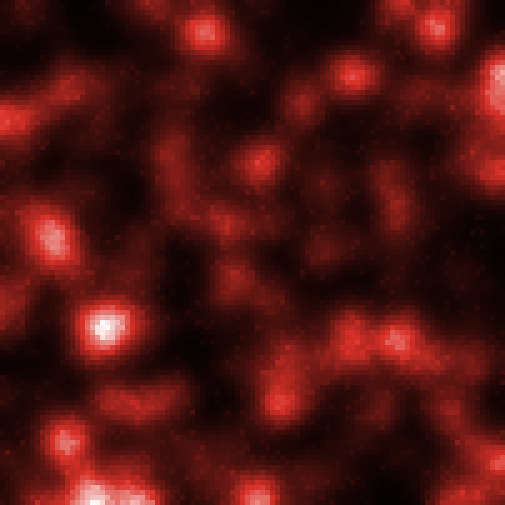
\includegraphics[width=0.45\textwidth]{Figures/PartII/Modeling/UrbanGrowth/ex0}\hspace{0.5cm}
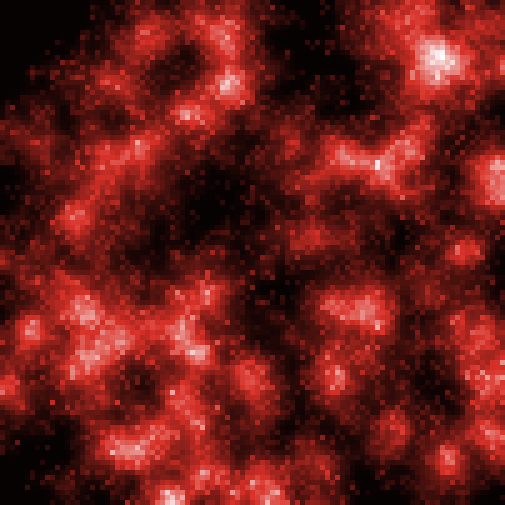
\includegraphics[width=0.45\textwidth]{Figures/PartII/Modeling/UrbanGrowth/ex1}\\
\medskip
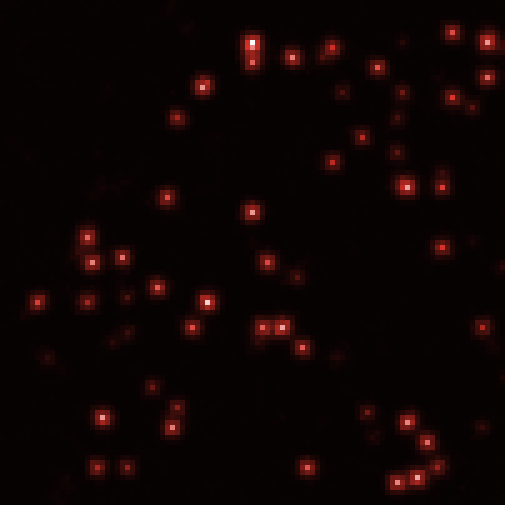
\includegraphics[width=0.45\textwidth]{Figures/PartII/Modeling/UrbanGrowth/ex2}\hspace{0.5cm}
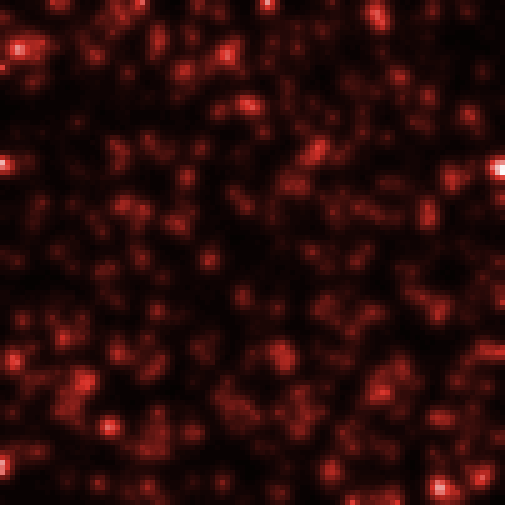
\includegraphics[width=0.45\textwidth]{Figures/PartII/Modeling/UrbanGrowth/ex3}\\\medskip
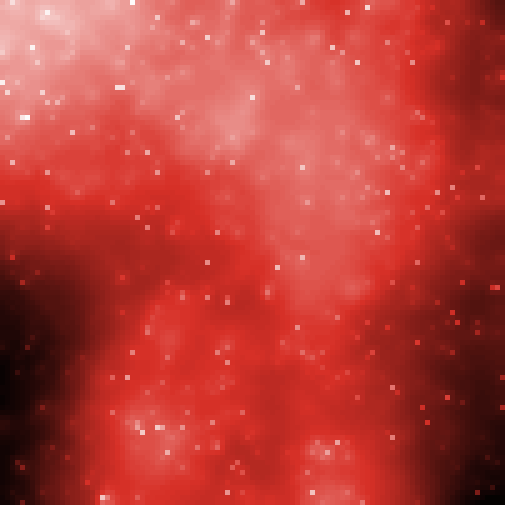
\includegraphics[width=0.45\textwidth]{Figures/PartII/Modeling/UrbanGrowth/ex4}\hspace{0.5cm}
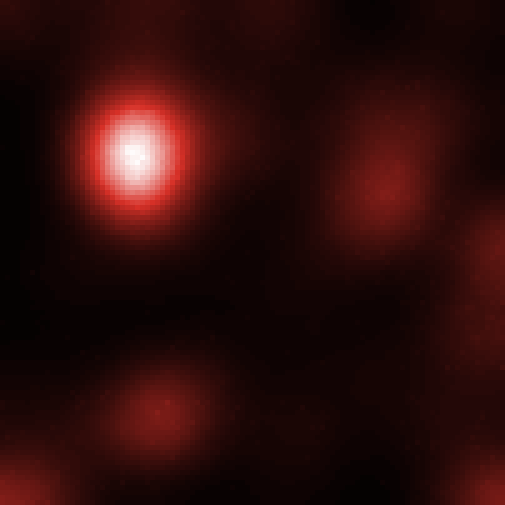
\includegraphics[width=0.45\textwidth]{Figures/PartII/Modeling/UrbanGrowth/ex5}\\\medskip
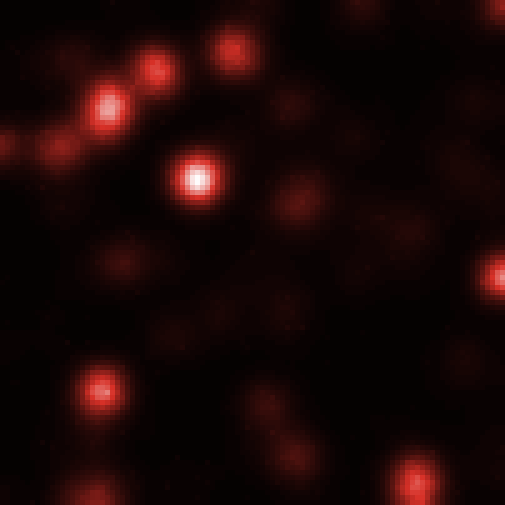
\includegraphics[width=0.45\textwidth]{Figures/PartII/Modeling/UrbanGrowth/ex6}\hspace{0.5cm}
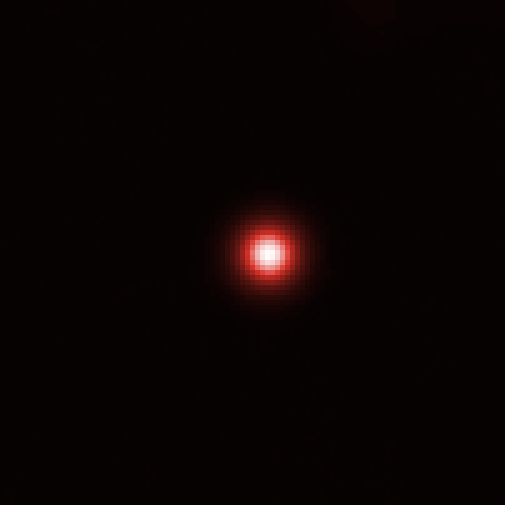
\includegraphics[width=0.45\textwidth]{Figures/PartII/Modeling/UrbanGrowth/ex7}\\
\caption[Generated Density urban shapes]{Example of the variety of generated urban shapes}
\label{fig:densitygeneration}
\end{figure}
%%%%%%%%%%%%




\subsubsection{Model Behavior}


\paragraph{Convergence - internal model validation}

%convergence properties of indicators ; number of repetitions needed for consistence of results. [histograms and stats of $\sigma$ %TODO]

Indicators show good convergence property and bimodal statistical distribution for cumulated points in the parameter space confirm the existence of superposed regimes : gaussian distribution gives stationary configurations, whereas inverse log-normal distribution are close to real data shape and correspond to non-stationary regime. For one point and a large number of repetitions, we find that 50 repetitions are enough to obtain a 95\% confidence interval smaller than $\sigma$ around indicator mean. 

\paragraph{Exploration of parameter space}

%Grid, then LHS explorations.

Parameter space is explored using a grid in first experiments, than a Latin Hypercube Sampling exploration. Parameter bounds are $\alpha \in [0.2,2],\beta \in [0,0.1],n_d \in \{0,\ldots , 4\}, N_G \in [500,3000], P_m \in [2000,100000]$. Fig.\ref{fig:densityscatter} shows the result. We also use the parameter space exploration algorithm~\cite{10.1371/journal.pone.0138212} implemented in OpenMole, and obtain in Fig.~\ref{fig:densitypse} the lower bound in Moran-entropy plan, that unexpectedly exhibit a scaling relationship that we aim to explore further.


%%%%%%%%%%%%
\begin{figure}
\hspace{-2cm}
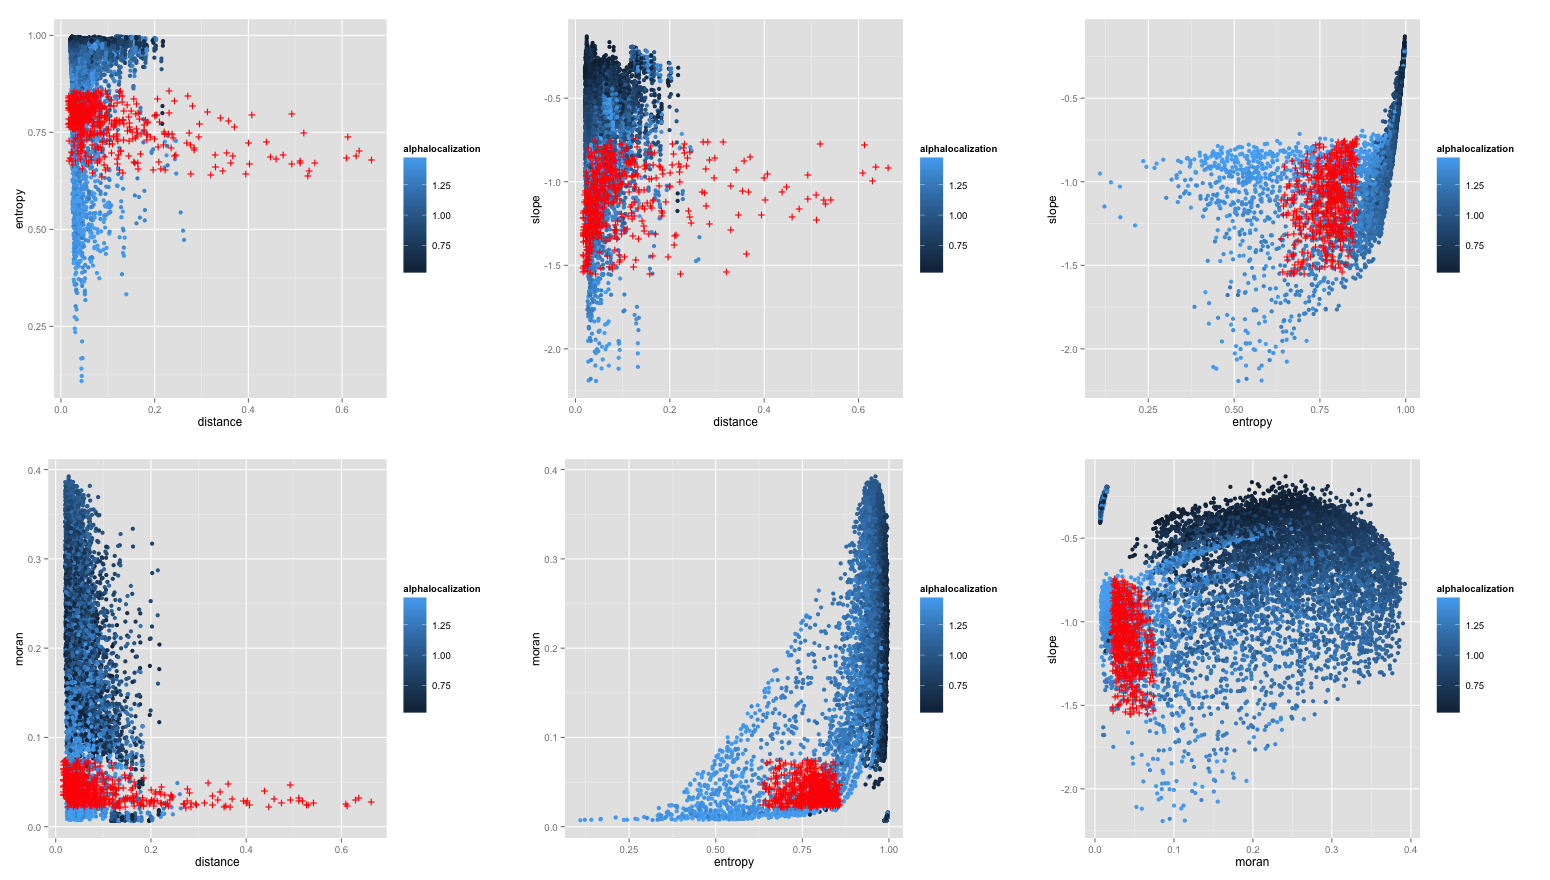
\includegraphics[width=1.4\textwidth]{Figures/PartII/Modeling/UrbanGrowth/all_alphaLoc}
\caption[LHS exploration of density model]{Scatterplots of indicators distribution in an hypercube of the parameter space. We show here the influence of one parameter (localization exponent $\alpha$). Red points correspond to real data.}
\label{fig:densityscatter}
\end{figure}
%%%%%%%%%%%%



%%%%%%%%%%%%
\begin{figure}
%\hspace{-2cm}
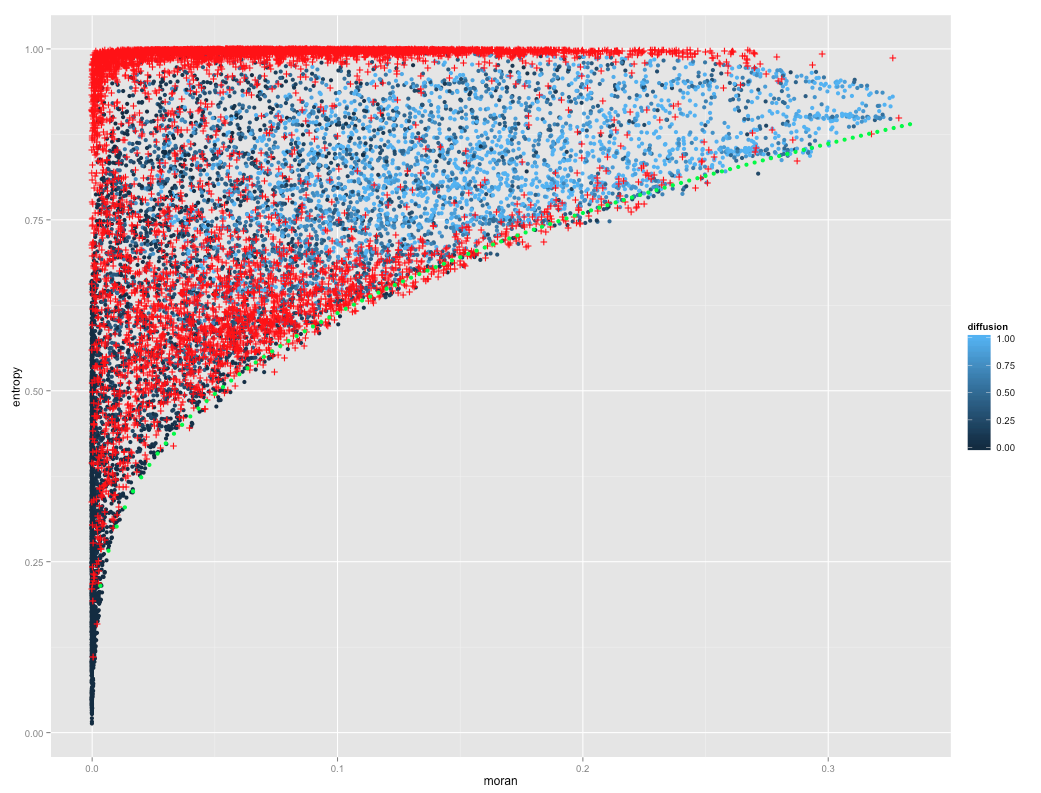
\includegraphics[width=\textwidth]{Figures/PartII/Modeling/UrbanGrowth/scaling_entropy_moran}
\caption[PSE exploration]{Scatterplots of Moran against Entropy, with blue points obtained with LHS and red with PSE exploration. Lower bound is in green.}
\label{fig:densitypse}
\end{figure}
%%%%%%%%%%%%



% Q : 3D plots as supp material ?

%Figure : on 2 first PC of morpho indicators, localization of typical shapes (monocentric city, polycentric city, diffuse rural settlements, aggregated rural settlements) / comparing generated shape with a typical real one

\paragraph{Statistical analysis}

%Regression indics = f(params) . TO BE DONE.
%interpretation ?

A statistical analysis (basic models) of indicator behaviors remains to be done and interpreted (one is done conjointly with network in paper corresponding to next section).

% 3.3 - Model Calibration
\subsubsection{Model Calibration}

% 3.3.1 - Real Data
\paragraph{Real Data}

%% Data source (density grid), computation methodology [comparison of sampling/smoothing to avoid bord effects ?] -> reals values of morpho indics on 50kmx50km grids, on all Europe.
%% + summary stats

%Figure : Distributions of indicators values for real dataset of european densities, computed on 50kmx50km grids, with 10km offset to avoid bord effects. [TODO : add log-normal/normal fits ? ]
%  -> cf Empirical Section

Empirical morphological measures for calibration are the one described in the empirical chapter, i.e. the calibration is done on morphological objectives (entropy, hierarchy, spatial auto-correlation, mean distance) against real values computed on the set of 50km sized grid extracted from european density grid~\cite{eurostat}.



\paragraph{Calibration Process}

We use a specific calibration process : a principal component analysis allows to maximize the cumulated distance between generated points and reals points. We select then the point cloud that overlaps real points in the (PC1,PC2) plan, given a distance threshold. Fig.~\ref{fig:densitycalib} shows the points we obtain for four different values of the threshold ranging from $10^{-6}$ to $10^{-3}$.



%%%%%%%%%%%%%%%
\begin{figure}
%\hspace{-2cm}
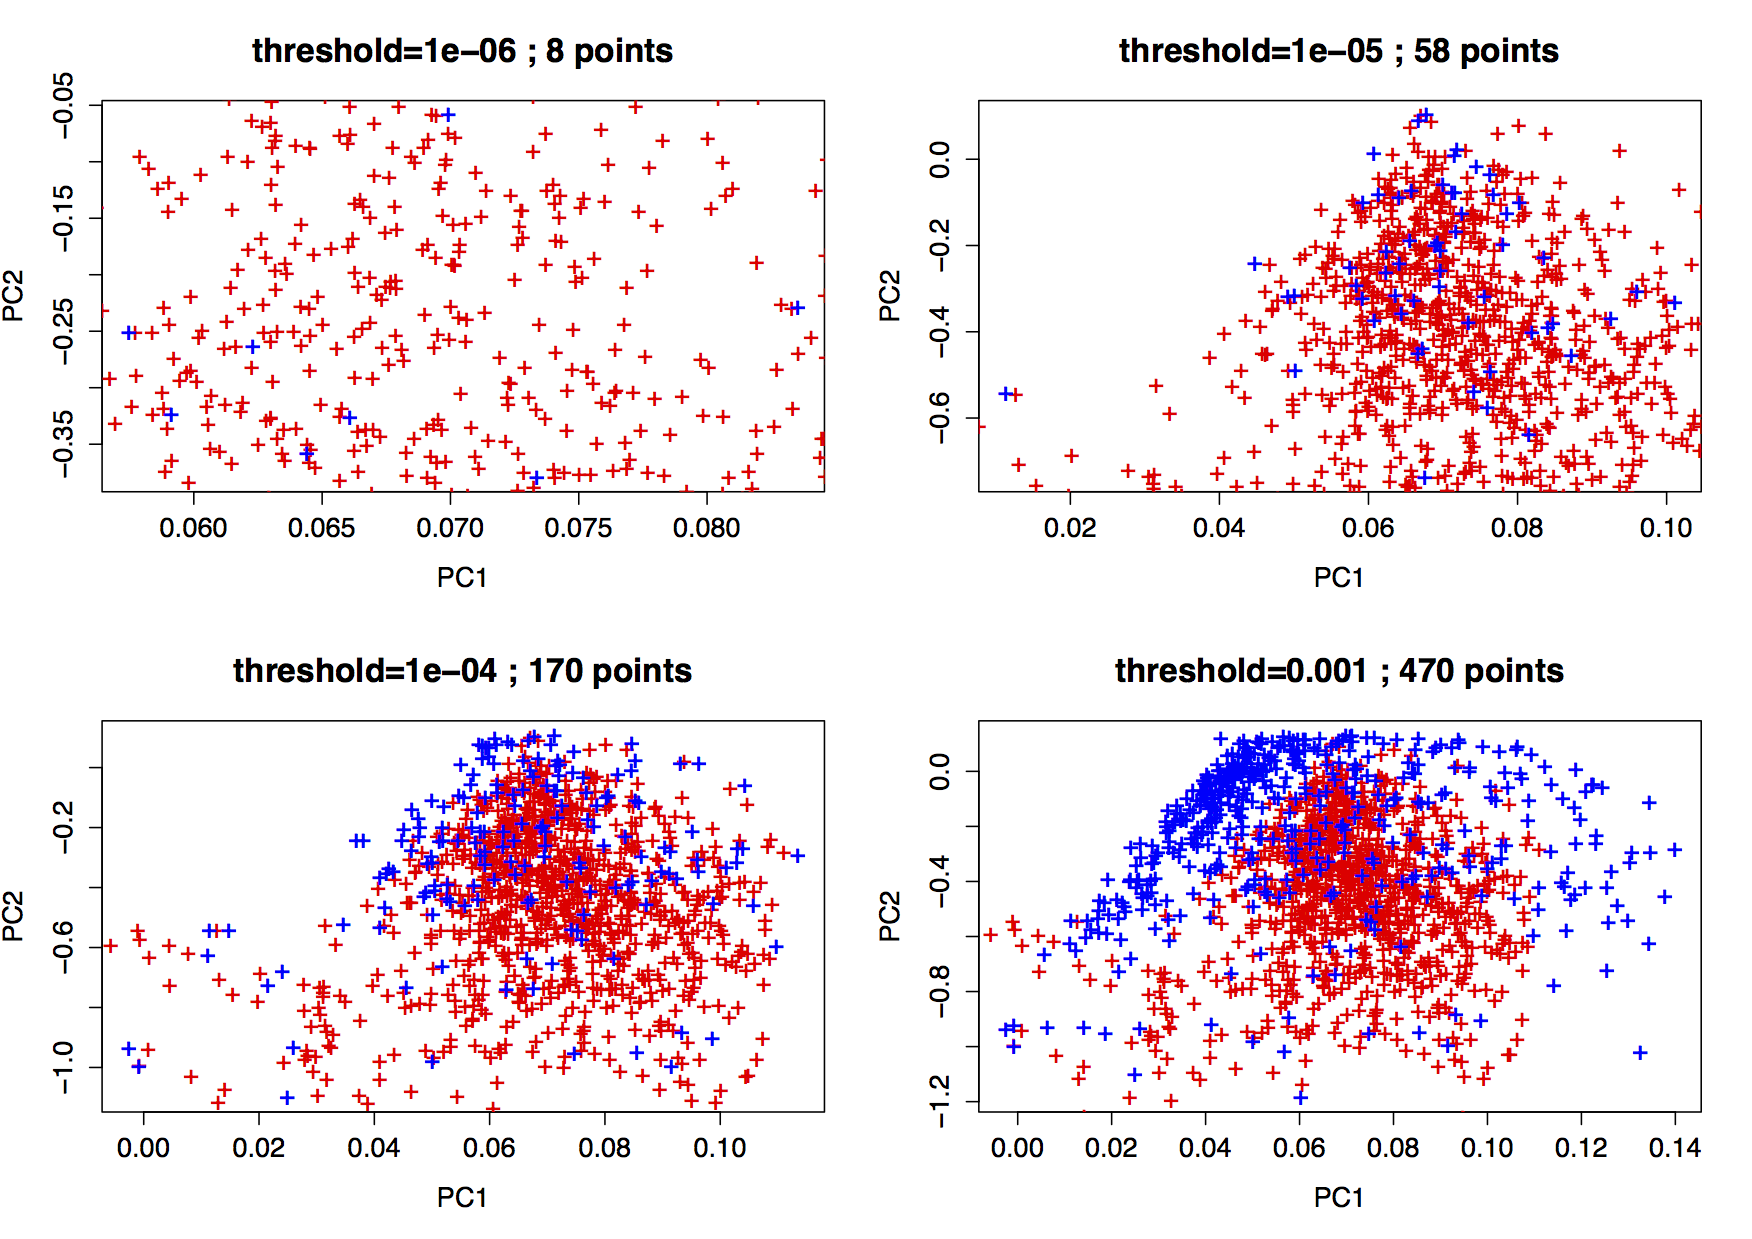
\includegraphics[width=\textwidth]{Figures/PartII/Modeling/UrbanGrowth/pcaDiff_thresholds}
\caption[Precise calibration of the model]{Precise calibration of the model. The principal component analysis is conducted to maximize the spread of the differences between real data and model output, i.e. on the set $\{\left|R_i - M_j\right|\}$ where $R_i$ is the set of real points, $M_j$ the set of model outputs. We select then the overlapping cloud at threshold $\theta$, by taking models output closer to real point cloud than $\theta$ in the (PC1,PC2) plan.}
\label{fig:densitycalib}
\end{figure}
%%%%%%%%%%%%%%



% 3.3.3 - Calibration Results
\subsubsection{Calibration refinement}

We plan in further work to extract the exact parameter space covering all real situations and provide interpretation of its shape (correlations between parameters). Its volume in different directions should give the relative importance of parameters.

%[possible development : application of Calibration Profile algo to check relative influence of parameters + ad hoc linear algebra on regression of 3.2.3 to do the same]




\subsection{Discussion}

\subsubsection{Thematic interpretation of growth behavior}

We still need to interpret the positions of typical shapes within parameter space in order to confirm the thematic interpretation of parameters. Depending on results of calibration refinement, we may obtain necessary and sufficient parameters to explain growth at this scale and a corresponding interpretation.

\subsubsection{Integration into a multi-scale growth model}

It could be possible to couple this model with a Gibrat (or Favaro-pumain) at Europa scale (macro) (with addition of consistence on migration constraints), where meso growth rates which were exogenous before are top-down determined, and bottom-up feedback is done through local aggregation level, influence importance of each area.


%%%%%
%% 4.3 - Methodological application ?
%%%%% -> maybe out of scope here ?

% -> Accurately calibrated spatialized urban growth model, can reproduce any (european) urban pattern.
% -> interpretation of parameter influence ; effective independant dimensions of the urban system at this scale.


In conclusion, this first modeling step provide an accurately calibrated spatial urban growth model at the mesoscopic scale that can reproduce any European urban pattern in terms of urban form. Further work is needed for an interpretation of parameter influence and the determination of effective independent dimensions of the urban system at this scale. We will use this model for other purposes in the following.

















%----------------------------------------------------------------------------------------


\newpage


% DO NOT INSERT FINANCIAL EXAMPLE ! 

\section{Correlated generation of territorial configurations}



This section aims to explore the sequential coupling between previous model of density generation and an heuristic of network growth. We explore therein the feasible space of correlations between network measures and morphological measures.% This work was initially presented as a methodological investigation in 


%%%%%%%%%%%%%%%%%%%%%%
\subsection{Correlated geographical data of density and network}


%%%%%%%%%%%%%%%%%%%%%%
\subsubsection{Context}


The use of synthetic data in geography is generally directed towards the generation of synthetic populations within agent-based models (mobility, \emph{LUTI} models)~\cite{pritchard2009advances}. We can make a weak link with some Spatial Analysis techniques. The extrapolation of a continuous spatial field from a discrete spatial sample through a kernel density estimation for example can be understood as the creation of a synthetic dataset (even if it is not generally the initial view, as in Geographically Weighted Regression~\cite{brunsdon1998geographically} in which variable size kernels do not interpolate data \emph{stricto sensu} but extrapolate abstract variables representing interaction between explicit variables). In the field of modeling in quantitative geography, \emph{toy-models} or hybrid models require a consistent initial spatial configuration. A set of possible initial configurations becomes a synthetic dataset on which the model is tested. The first Simpop model~\cite{sanders1997simpop}, precursor of a large family of models later parametrized with real data, could enter that frame but was studied on an unique synthetic spatialization. Similarly underlined was the difficulty to generate an initial transportation infrastructure in the case of the SimpopNet model~\cite{schmitt2014modelisation} although it was admitted as a cornerstone of knowledge on the behavior of the model. A systematic control of spatial configuration effects on the behavior of simulation models was only recently proposed~\cite{cottineau2015revisiting}, approach that can be interpreted as a statistical control on spatial data. The aim is to be able to distinguish proper effects due to intrinsic model dynamics from particular effects due to the geographical structure of the case study. Such results are essential for the validation of conclusions obtained with modeling and simulation practices in quantitative geography.



%%%%%%%%%%%%%%%%%%%%%%
\subsubsection{Formalization}

We propose in our case to generate territorial systems summarized in a simplified way as a spatial population density $d(\vec{x})$ and a transportation network $n(\vec{x})$. Correlations we aim to control are correlations between urban morphological measures and network measures. The question of interactions between territories and networks is already well-studied~\cite{offner1996reseaux} but stays highly complex and difficult to quantify~\cite{offner1993effets}. A dynamical modeling of implied processes should shed light on these interactions (\cite{bretagnolle:tel-00459720}, p. 162-163). We develop in that frame a \emph{simple} coupling (i.e. without any feedback loop) between a density distribution model and a network morphogenesis model.



\paragraph{Density model}

The density model is the model described and explored in the previous section. We use it for the conditional generation of network.


\paragraph{Network model}


On the other hand, we are able to generate a planar transportation network by a model $N$, at a similar scale and given a density distribution. Because of the conditional nature to the density of the generation process, we will first have conditional estimators for network indicators, and secondly natural correlations between network and urban shapes should appear as processes are not independent. The nature and modularity of these correlations as a function of model parameters are still to determine by exploration of the coupled model.



The heuristic network generation procedure is the following :
\begin{enumerate}
\item A fixed number $N_c$ of centers that will be first nodes of the network si distributed given density distribution, following a similar law to the aggregation process, i.e. the probability to be distributed in a given patch is $\frac{(P_i/P)^{\alpha}}{\sum (P_i/P)^{\alpha}}$. Population is then attributed according to Voronoi areas of centers, such that a center cumulates population of patches within its extent.
\item Centers are connected deterministically by percolation between closest clusters : as soon as network is not connected, two closest connected components in the sense of minimal distance between each vertices are connected by the link realizing this distance. It yields a tree-shaped network.
\item Network is modulated by potential breaking in order to be closer from real network shapes. More precisely, a generalized gravity potential between two centers $i$ and $j$ is defined by
\[
V_{ij}(d) = \left[ (1 - k_h) + k_h \cdot \left( \frac{P_i P_j}{P^2} \right)^{\gamma} \right]\cdot \exp{\left( -\frac{d}{r_g (1 + d/d_0)} \right)}
\]
where $d$ can be euclidian distance $d_{ij}=d(i,j)$ or network distance $d_N(i,j)$, $k_h \in [0,1]$ a weight to modulate role of populations, $\gamma$ giving shape of the hierarchy across population values, $r_g$ characteristic interaction distance and $d_0$ distance shape parameter.
\item A fixed number $K\cdot N_L$ of potential new links is taken among couples having greatest euclidian distance potential ($K=5$ is fixed).
\item Among potential links, $N_L$ are effectively realized, that are the one with smallest rate $\tilde{V}_{ij} = V_{ij}(d_N)/V_{ij}(d_{ij})$. At this stage only the gap between euclidian and network distance is taken into account : $\tilde{V}_{ij}$ does indeed not depend on populations and is increasing with $d_N$ at constant $d_{ij}$.
\item Planarity of the network is forced by creation of nodes at possible intersections created by new links.
\end{enumerate}



We insist on the fact that the network generation procedure is entirely heuristic and result of thematic assumptions (connected initial network, gravity-based link creation) combined with trial-and-error during first explorations. Other model types could be used as well, such biological self-generated networks~\cite{tero2010rules}, local network growth based on geometrical constraints optimization~\cite{barthelemy2008modeling}, or a more complex percolation model than the initial one that would allow the creation of loops for example. We could thus in the frame of a modular architecture, in which the choice between different implementations of a functional brick can be seen as a meta-parameter~\cite{cottineau2015incremental}, choose network generation function adapted to a specific need (as e.g. proximity to real data, constraints on output indicators, variety if generated forms, etc. ).




%  must do a computational benchmark for various network generation models ; calibrated on real data. -> cf network generation section.

\paragraph{Parameter space}

Parameter space for the coupled model\footnote{Weak coupling allows to limit the total number of parameters as a strong coupling would involve retroaction loops and consequently associated parameters to determine their structure and intensity. In order to diminish it, an integrated model would be preferable to a strong coupling, what is slightly different in the sense where it is not possible in the integrated model to freeze one of the subsystems to obtain a model of the other subsystem that would correspond to the non-coupled model.} is constituted by density generation parameters $\vec{\alpha}_D = (P_m/N_G , \alpha,\beta , n_d)$ (we study for the sake of simplicity the rate between population and growth rate instead of both varying, i.e. the number of steps needed to generate the distribution) and network generation parameters $\vec{\alpha}_N=(N_C,k_h,\gamma , r_g , d_0)$. We denote $\vec{\alpha} = (\vec{\alpha}_D,\vec{\alpha}_N)$. 




% these notion of weak / strong coupling are not enough developed or reference-based. ---> find it in literature ? not sure exists like that. --> integarte it in theoretical paper ? or separate working paper.

\paragraph{Indicators}

Urban form and network structure are quantified by numerical indicators in order to modulate correlations between these. Morphology is defined as a vector $\vec{M}=(r,\bar{d},\varepsilon,a)$ giving spatial auto-correlation (Moran index), mean distance, entropy and hierarchy (see~\cite{le2015forme} for a precise definition of these indicators). Network measures $\vec{G} = (\bar{c},\bar{l},\bar{s},\delta)$ are with network denoted $(V,E)$
\begin{itemize}
\item Mean centrality $\bar{c}$ defined as average \emph{betweeness-centrality} (normalized in $[0,1]$) on all links.
\item Mean path length $\bar{l}$ given by $\frac{1}{d_m}\frac{2}{|V|\cdot (|V|-1)}\sum_{i<j}d_N(i,j)$ with $d_m$ normalization distance taken here as world diagonal $d_m=\sqrt{2}N$.
\item Mean network speed~\cite{banos2012towards} which corresponds to network performance compared to direct travel, defined as $\bar{s} = \frac{2}{|V|\cdot (|V|-1)}\sum_{i<j}{\frac{d_{ij}}{d_N(i,j)}}$.
\item Network diameter $\delta = \max_{ij}d_N(i,j)$.
\end{itemize}




\paragraph{Covariance and correlation}

We study the cross-correlation matrix $\Covb{\vec{M}}{\vec{G}}$ between morphology and network. We estimate it on a set of $n$ realizations at fixed parameter values $(\vec{M}\left[D(\vec{\alpha})\right],\vec{G}\left[N(\vec{\alpha})\right])_{1\leq i\leq n}$ with standard unbiased estimator. We estimate correlation with associated Pearson estimator. 



%%%%%%%%%%%%%%%%%%%%%%
\subsubsection{Implementation}


Coupling of generative models is done both at formal and operational levels. We interface therefore independent implementations. The OpenMole software~\cite{reuillon2013openmole} for intensive model exploration offers for that the ideal frame thanks to its modular language allowing to construct \emph{workflows} by task composition and interfacing with diverse experience plans and outputs. For operational reasons, density model is implemented in \texttt{scala} language as an OpenMole \texttt{plugin}, whereas network generation is implemented in agent-oriented language \texttt{NetLogo}~\cite{wilensky1999netlogo} because of its possibilities for interactive exploration and heuristic model construction. Source code is available for reproducibility on project repository\footnote{at \texttt{https://github.com/JusteRaimbault/CityNetwork/tree/master/Models/Synthetic}}.





%%%%%%%%%%%%%%
\begin{figure}

\subfloat[]{%[t]{0.35\linewidth}
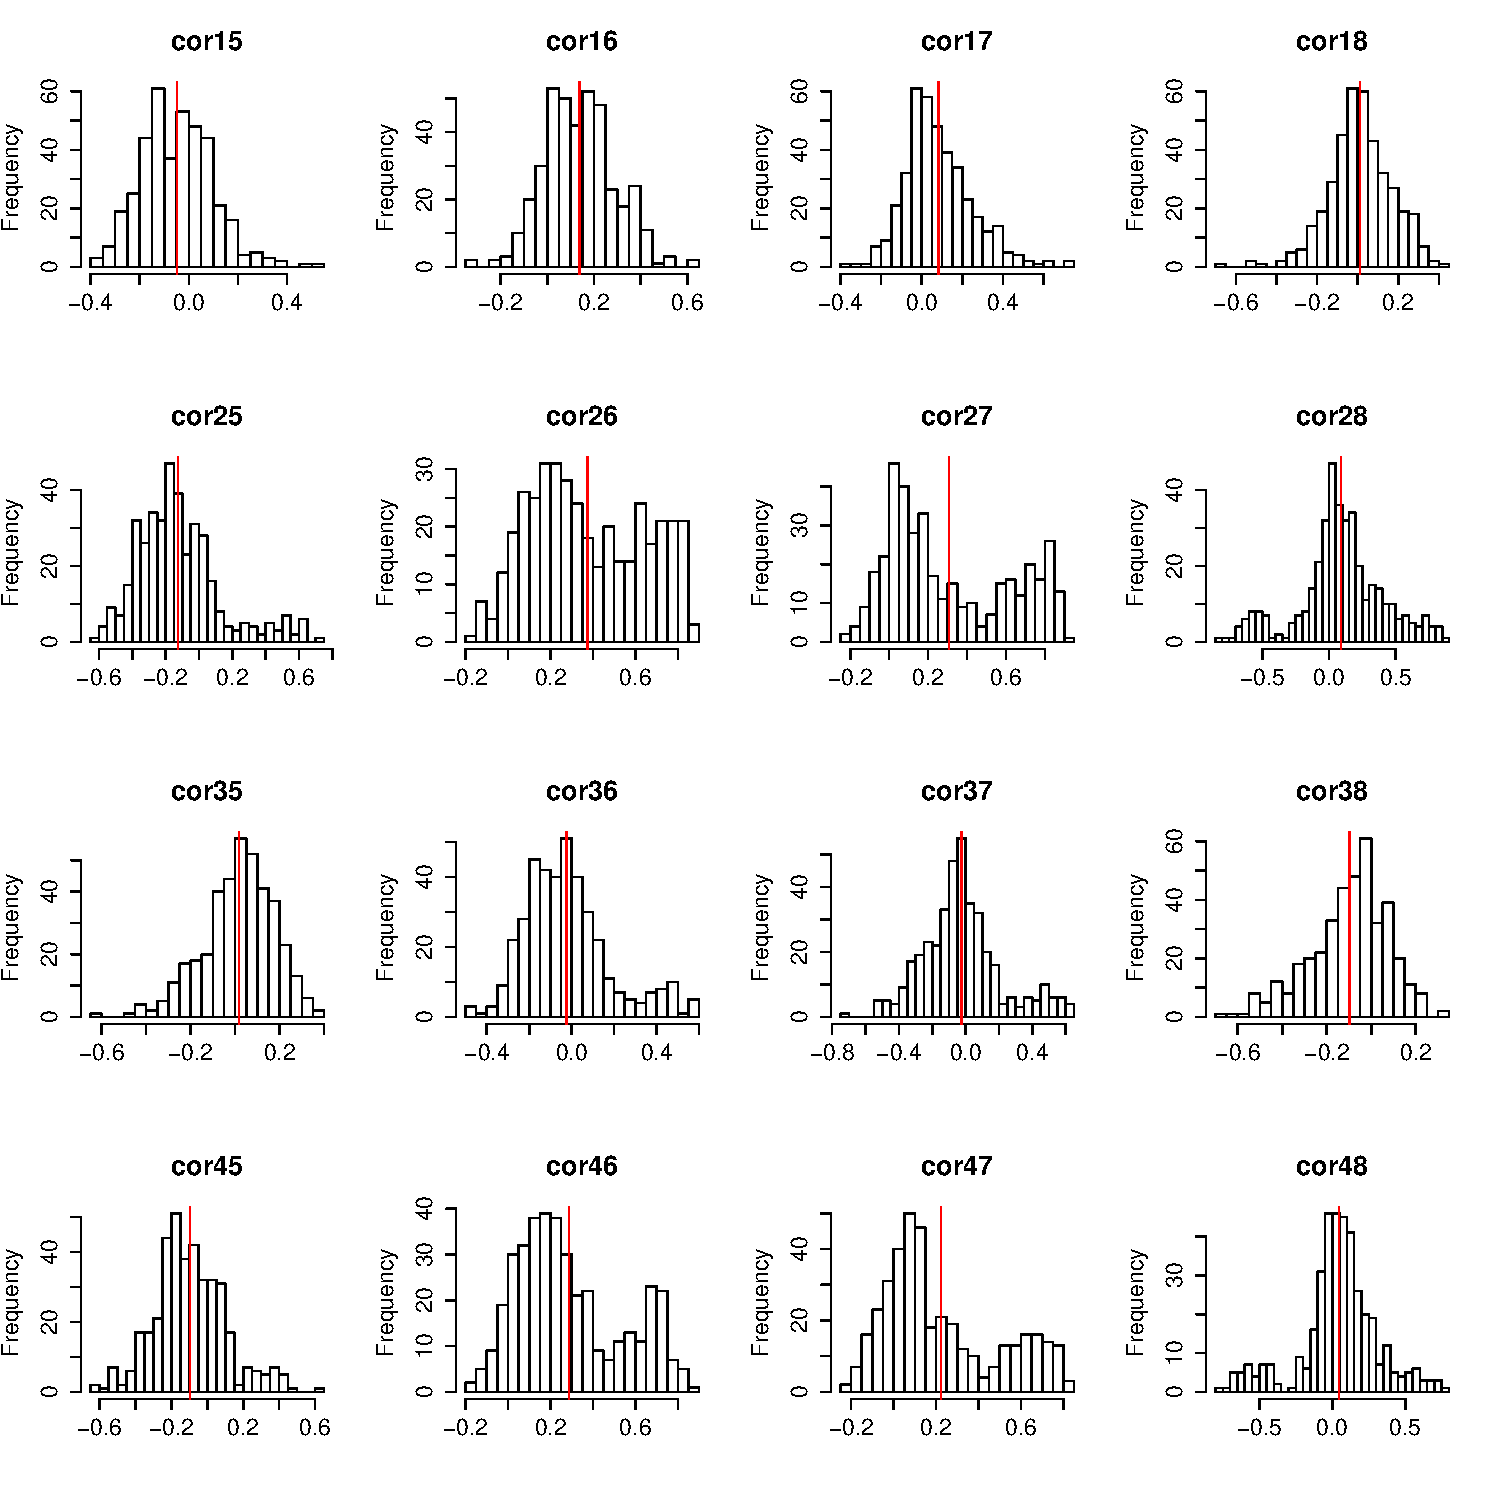
\includegraphics[width=0.35\textwidth]{Figures/PartII/Modeling/CorrelatedData/hist_crossCorMat_breaks30}
%\caption{}
}
\subfloat[]{%[t]{0.23\linewidth}
\vspace{-6.5cm}
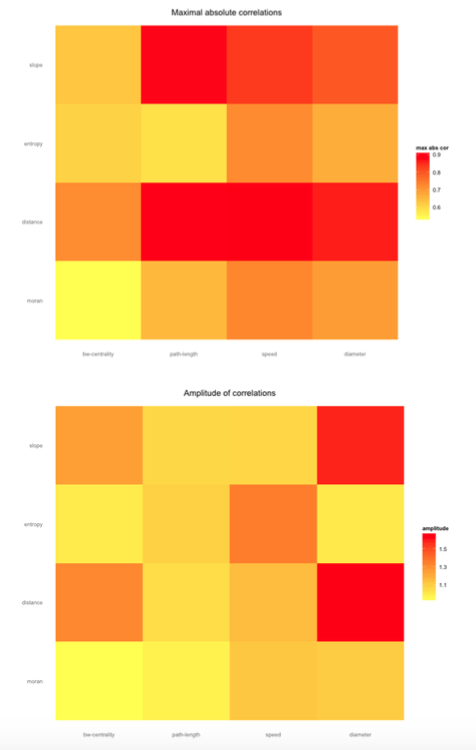
\includegraphics[width=0.23\textwidth]{Figures/PartII/Modeling/CorrelatedData/heatmaps}
}
\subfloat[]{%[t]{0.4\linewidth}
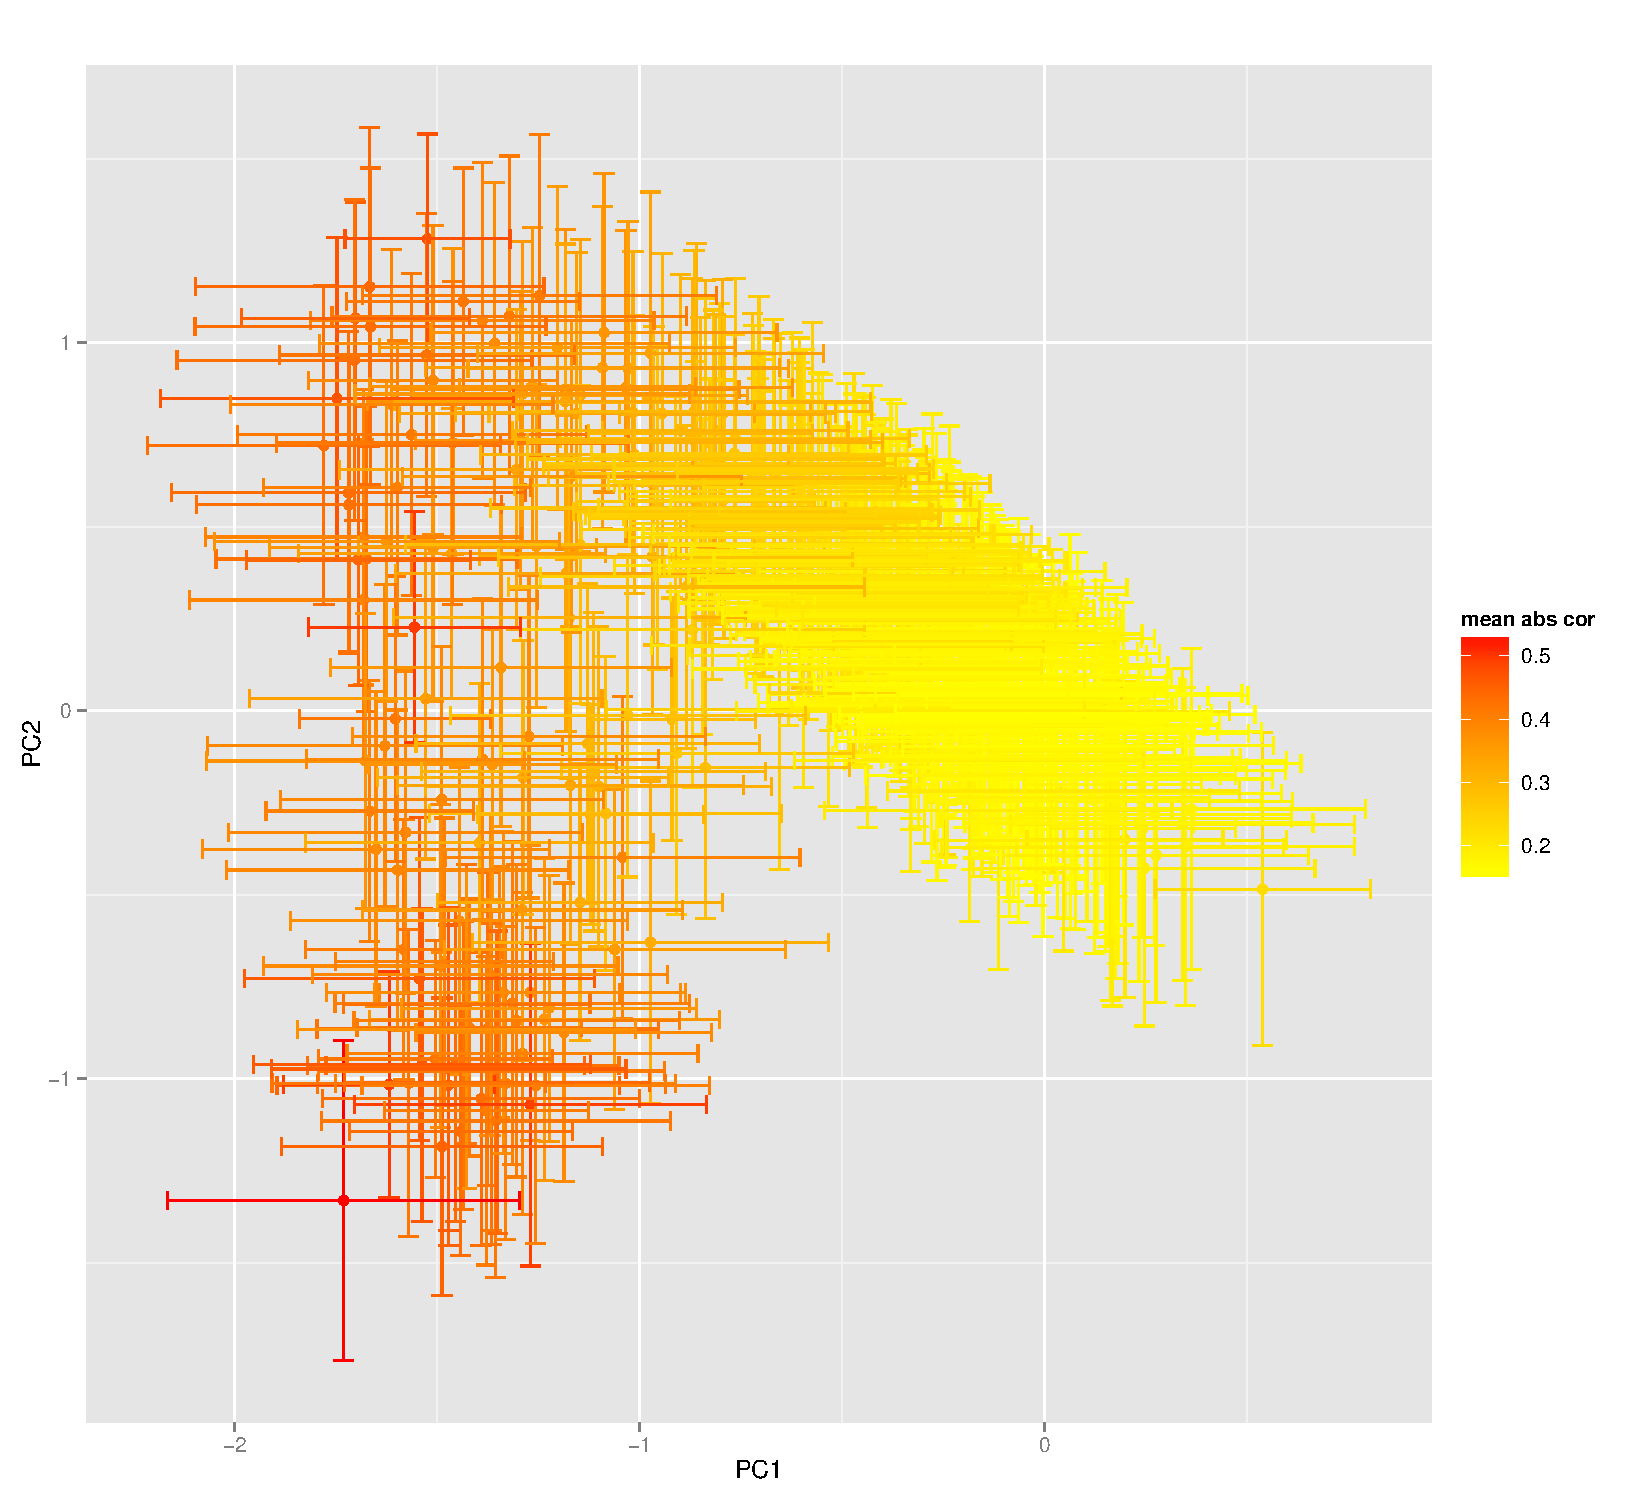
\includegraphics[width=0.4\textwidth]{Figures/PartII/Modeling/CorrelatedData/pca_meanAbsCor_errorBars}
}\\
\subfloat[]{%[t]{0.54\linewidth}
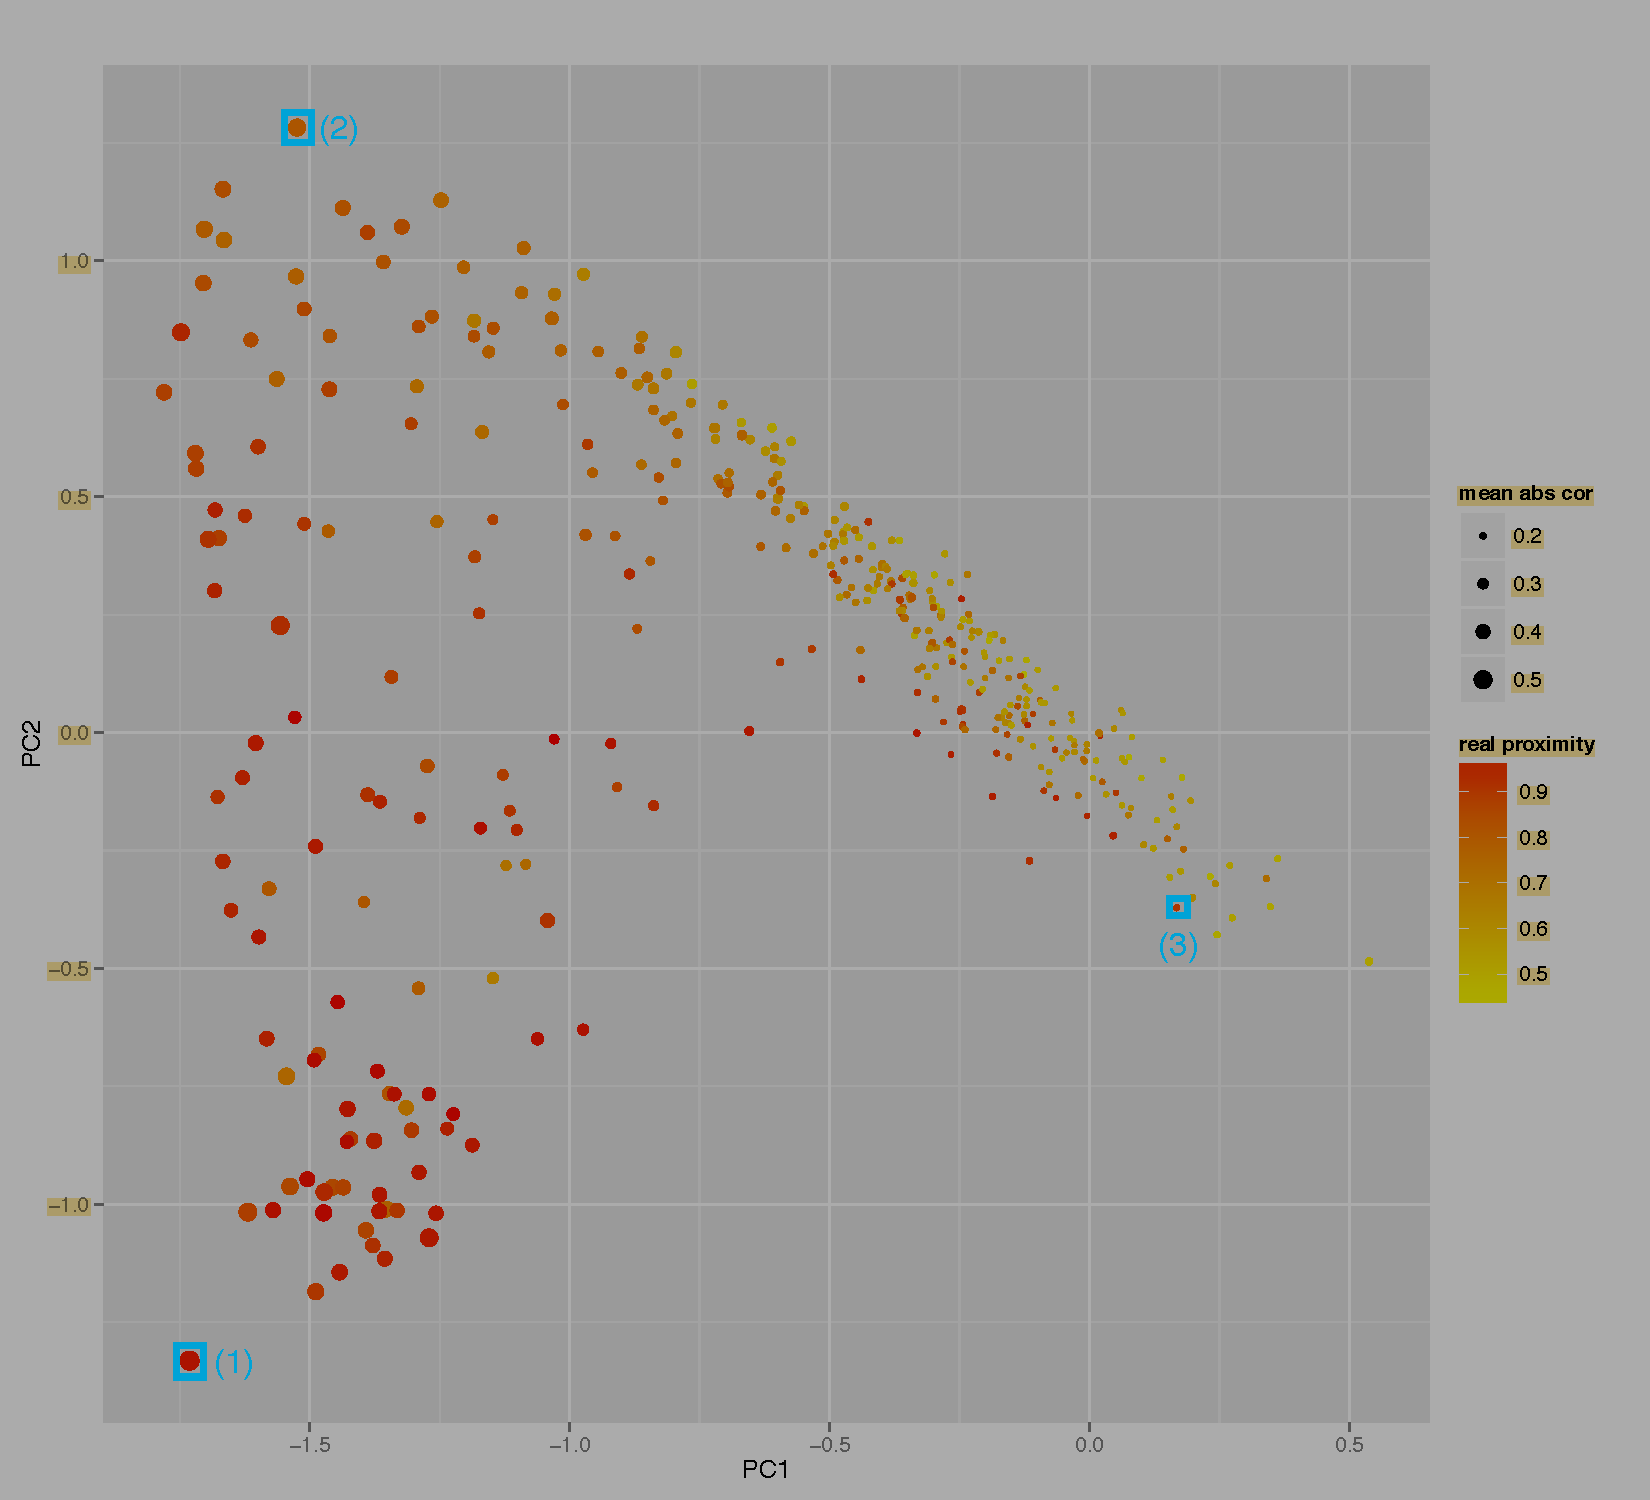
\includegraphics[width=\textwidth]{Figures/PartII/Modeling/CorrelatedData/pca_realDistCol_meanAbsCorSize_withSpecificPoints}
}
\subfloat[]{%[t]{0.45\linewidth}
\vspace{-8.3cm}
}

\caption[Exploration of feasible space for correlations between urban morphology and network structure]{\footnotesize\textbf{Exploration of feasible space for correlations between urban morphology and network structure | } \textbf{(a)} Distribution of crossed-correlations between vectors $\vec{M}$ of morphological indicators (in numbering order Moran index, mean distance, entropy, hierarchy) and $\vec{N}$ of network measures (centrality, mean path length, speed, diameter). \textbf{(b)} Heatmaps for amplitude of correlations, defined as $a_{ij}=\max_k{\rho_{ij}^{(k)}}-\min_k{\rho_{ij}^{(k)}}$ and maximal absolute correlation, defined as $c_{ij}=\max_k\left| \rho_{ij}^{k} \right|$. \textbf{(c)} Projection of correlation matrices in a principal plan obtained by Principal Component Analysis on matrix population (cumulated variances: PC1=38\%, PC2=68\%). Error bars are initially computed as 95\% confidence intervals on each matrix element (by standard Fisher asymptotic method), and upper bounds after transformation are taken in principal plan. Scale color gives mean absolute correlation on full matrices. \textbf{(d)} Representation in the principal plan, scale color giving proximity to real data defined as $1 - \min_r \norm{\vec{M}-\vec{M}_r}$ where $\vec{M}_r$ is the set of real morphological measures, point size giving mean absolute correlation.}
\label{fig:densnwcor}
\end{figure}
%%%%%%%%%%%%%%


%%%%%%%%%%%%%%
\begin{figure}
\centering

   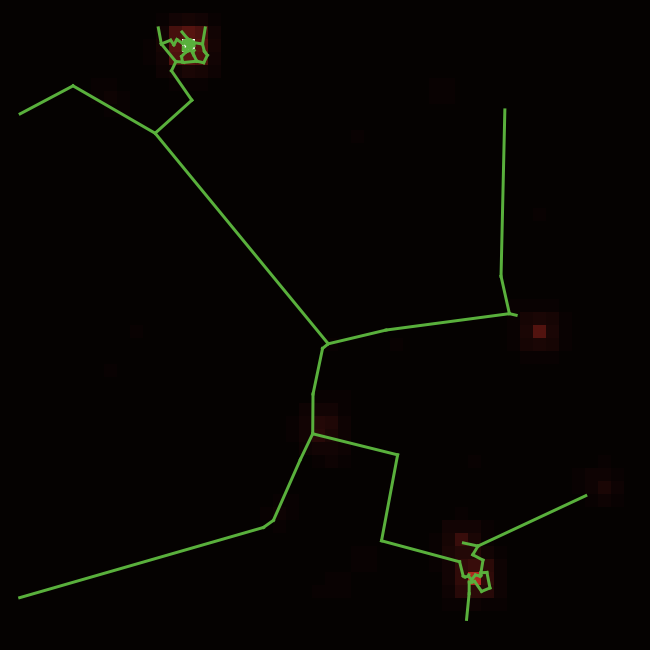
\includegraphics[width=0.45\textwidth]{Figures/PartII/Modeling/CorrelatedData/configs/1_param71861_seed0}
   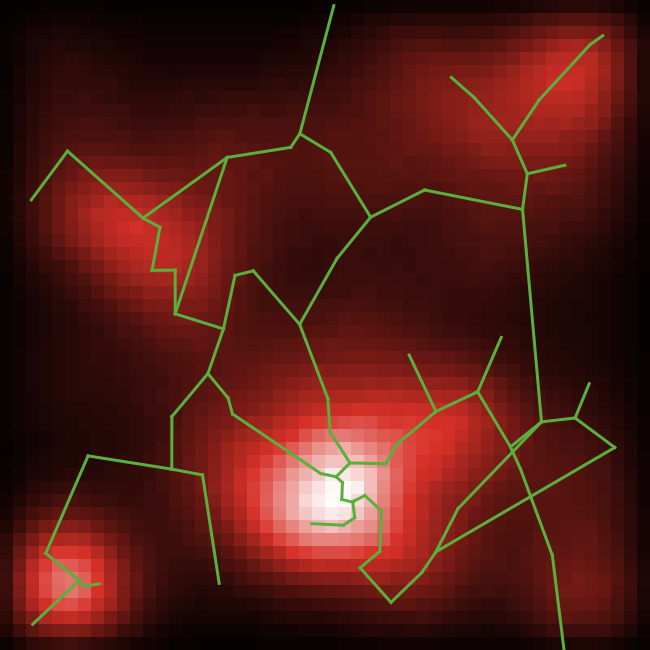
\includegraphics[width=0.45\textwidth]{Figures/PartII/Modeling/CorrelatedData/configs/2_param71913_seed10}\\
   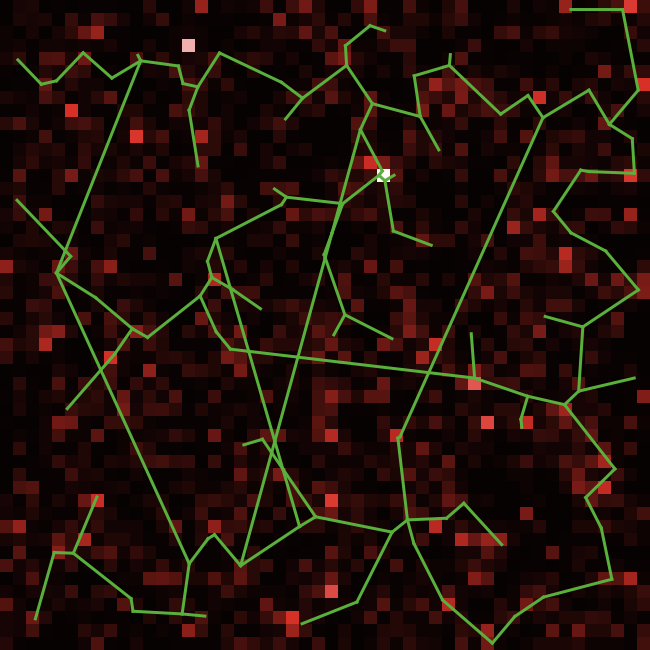
\includegraphics[width=0.45\textwidth]{Figures/PartII/Modeling/CorrelatedData/configs/3_param71918_seed0}
   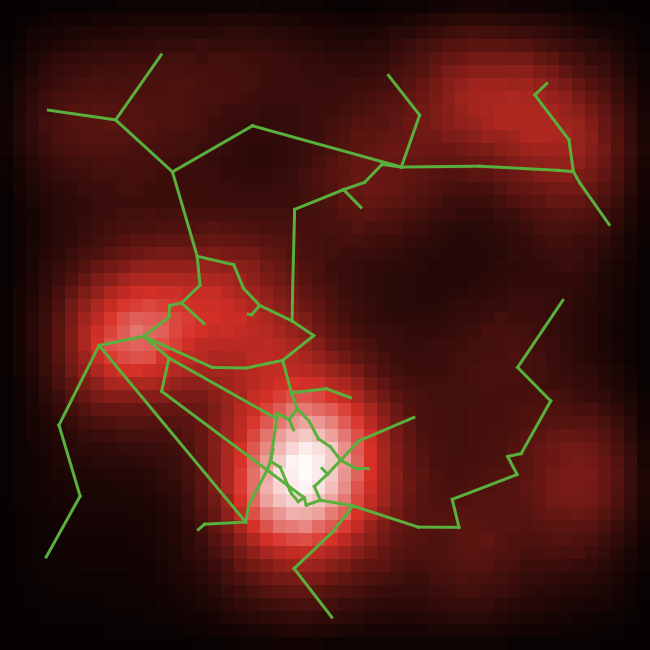
\includegraphics[width=0.45\textwidth]{Figures/PartII/Modeling/CorrelatedData/configs/4_param71945_seed0}
\caption[Examples of generated coupled configurations]{Configurations obtained for parameters giving the four emphasized points in (d), in order from left to right and top to bottom. We recognize polycentric city configurations (2 and 4), diffuse rural settlements (3) and aggregated weak density area (1). See appendice for exhaustive parameter values, indicators and corresponding correlations. For example $\bar{d}$ is highly correlated with $\bar{l},\bar{s}$ ($\simeq$0.8) in (1) but not for (3) although both correspond to rural environments ; in the urban case we observe also a broad variability : $\rho[\bar{d},\bar{c}]\simeq 0.34$ for (4) but $\simeq-0.41$ for (2), what is explained by a stronger role of gravitation hierarchy in (2) $\gamma=3.9,k_h=0.7$ (for (4), $\gamma=1.07,k_h=0.25$), whereas density parameters are similar.}
\end{figure}
%%%%%%%%%%%%%%





%%%%%%%%%%%%%%%%%%%%%%
\subsubsection{Results}

The study of density model alone is developed in~\cite{raimbault2016calibration}. It is in particular calibrated on European density grid data, on 50km width square areas with 500m resolution for which real indicator values have been computed on whole Europe. Furthermore, a grid exploration of model behavior yields feasible output space in reasonable parameters bounds (roughly $\alpha \in [0.5,2],N_G\in [500,3000], P_m \in [10^4,10^5],\beta\in [0,0.2], n_d \in \{ 1, \ldots , 4\}$). The reduction of indicators space to a two dimensional plan through a Principal Component Analysis (variance explained with two components $\simeq 80\%$) allows to isolate a set of output points that covers reasonably precisely real point cloud. It confirms the ability of the model to reproduce morphologically the set of real configurations.



% NOT NEEDED - TOO MUCH INFORMATION - ?
%%%%%%%%%%%%%%%%
%\begin{figure}
% figure : density example, exploration and calibration ?
%\end{figure}
%%%%%%%%%%%%%%%%

At given density, the conditional exploration of network generation model parameter space suggest a good flexibility on global indicators $\vec{G}$, together with good convergence properties. For a precise study of model behavior, see appendice giving regressions analysis capturing the behavior of coupled model. In order to illustrate synthetic data generation method, the exploration has been oriented towards the study of cross-correlations.


%A densité donnée, l'exploration de l'espace des paramètres du modèle de réseau suggèrent une assez bonne flexibilité sur des indicateurs globaux $\vec{G}$, ainsi que de bonnes propriétés de convergence. Pour une étude du comportement précis, voir l'appendice donnant les regressions traduisant le comportement du modèle couplé. Dans le but d'illustrer la méthode de génération de données synthétiques, l'exploration a été orientée vers l'étude des correlations.


Given the large relative dimension of parameter space, an exhaustive grid exploration is not possible. We use a Latin Hypercube sampling procedure with bounds given above for $\vec{\alpha}_D$ and for $\vec{\alpha}_N$, we take $N_C \in [50,120], r_g \in [1,100] , d_0 \in [0.1,10] , k_h \in [0,1] , \gamma \in [0.1,4],N_L\in [4,20]$. For number of model replications for each parameter point, less than 50 are enough to obtain confidence intervals at 95\% on indicators of width less than standard deviations. For correlations a hundred give confidence intervals (obtained with Fisher method) of size around 0.4, we take thus $n=80$ for experiments. Figure~\ref{fig:densnwcor} gives details of experiment results. Regarding the subject of correlated synthetic data generation, we can sum up the main lines as following :
\begin{itemize}
\item Empirical distributions of correlation coefficients between morphology and network indicators are not simple and some are bimodal (for example $\rho_{46}=\rho[r,\bar{l}]$  between Moran index and mean path length).
\item it is possible to modulate up to a relatively high level of correlation for all indicators, maximal absolute correlation varying between 0.6 and 0.9. Amplitude of correlations varies between 0.9 and 1.6, allowing a broad spectrum of values. Point cloud in principal plan has a large extent but is not uniform : it is not possible to modulate at will any coefficient as they stay themselves correlated because of underlying generation processes. A more refined study at higher orders (correlation of correlations) would be necessary to precisely understand degrees of freedom in correlation generation.
\item Most correlated points are also the closest to real data, what confirms the intuition and stylized fact of a strong interdependence in reality.
\item Concrete examples taken on particular points in the principal plan show that similar density profiles can yield very different correlation profiles.
\end{itemize}




%%%%%%%%%%%%%%
%\begin{table}
%regression analysis of param influence on correlations
%  -> Appendice.
%\end{table}
%%%%%%%%%%%%%%




\subsubsection{Possible developments}


This case study could be refined by extending correlation control method. A precise knowledge of $N$ behavior (statistical distributions on an exhaustive grid of parameter space) conditional to $D$ would allow to determine $N^{<-1>} | D$ and have more latitude in correlation generation. We could also apply specific exploration algorithms to reach exceptional configurations realizing an expected correlation level, or at least to obtain a better knowledge of the feasible space of correlations~\cite{10.1371/journal.pone.0138212}.




%%%%%%%%%%%%%%%%%%%%%%
\subsection{Discussion}
%%%%%%%%%%%%%%%%%%%%%%



%%%%%%%%%%%%%%%%%%%%%%
\subsubsection*{Scientific positioning}

% données hybrides au centre de la démarche d'exploration de modèle, analyse de sensitivité etc.

Our overall approach enters a particular epistemological frame. On the one hand the multidisciplinary aspect, and on the other hand the importance of empirical component through computational exploration methods, make this approach typical of Complex Systems science, as it is recalled by the roadmap for Complex Systems having a similar structure~\cite{2009arXiv0907.2221B}. It combines transversal research questions (horizontal integration of disciplines) with the development of heterogeneous multi-scalar approaches which encounter similar issues as the one we proposed to tackle (vertically integrated disciplines). The combination of empirical knowledge obtained from data mining, with knowledge obtained by modeling and simulation is generally central to the conception and exploration of multi-scalar heterogeneous models. Results presented here is an illustration of such an hybrid paradigm.




%%%%%%%%%%%%%%%%%%%%%%
\subsubsection*{Direct applications}


Starting from the second example which was limited to data generation, we propose examples of direct applications that should give an overview of the range of possibilities.

%En partant du deuxième exemple, qui s'est arrêté à la génération des données synthétiques, on peut proposer des pistes d'application directe qui donneront un aperçu de l'éventail des possibilités.

\begin{itemize}
\item Calibration of network generation component at given density, on real data for transportation network (typically road network given the shape of generated networks ; it should be straightforward to use OpenStreetMap open data\footnote{\texttt{https://www.openstreetmap.org}} that have a reasonable quality for Europe, at least for France~\cite{girres2010quality}, with however adjustments on generation procedure in order to avoid edge effects due its restrictive frame, for example by generating on an extended surface to keep only a central area on which calibration would be done) should theoretically allow to unveil parameter sets reproducing accurately existing configurations both for urban morphology and network shape. It could be then possible to derive a ``theoretical correlation'' for these, as an empirical correlation is according to some theories of urban systems not computable as a unique realization of stochastic processes is observed. Because of non-ergodicity of urban systems~\cite{pumain2012urban}, there are strong chances that involved processes are different across different geographical areas (or from an other point of view that they are in an other state of meta-parameters, i.e. in an other regime) and that their interpretation as different realizations of the same stochastic process makes no sense, the impossibility of covariation estimation following. By attributing a synthetic dataset similar to a given real configuration, we would be able to compute a sort of \emph{intrinsic correlation} proper to this configuration. As territorial configurations emerge from spatio-temporal interdependences between components of territorial systems, this intrinsic correlation emerges the same way, and its knowledge gives information on these interdependences and thus on relations between territories and networks.
\item As already mentioned, most of models of simulation need an initial state generated artificially as soon as model parametrization is not done completely on real data. An advanced model sensitivity analysis implies a control on parameters for synthetic dataset generation, seen as model meta-parameters~\cite{cottineau2015revisiting}. In the case of a statistical analysis of model outputs it provides a way to operate a second order statistical control.
\item We studied in the first example stochastic processes in the sense of random time-series, whereas time did not have a role in the second case. We can suggest a strong coupling between the two model components (or the construction of an integrated model) and to observe indicators and correlations at different time steps during the generation. In a dynamical spatial models we have because of feedbacks necessarily propagation effects and therefore the existence of lagged interdependences in space and time~\cite{pigozzi1980interurban}. It would drive our field of study towards a better understanding of dynamical correlations.
\end{itemize}




%%%%%%%%%%%%%%%%%%%%%%
\subsubsection*{Generalization}

We were limited to the control of first and second moments of generated data, but we could imagine a theoretical generalization allowing the control of moments at any order. However, as shown by the geographical example, the difficulty of generation in a concrete complex case questions the possibility of higher orders control when keeping a consistent structure model and a reasonable number of parameters. The study of non-linear dependence structures as proposed in~\cite{chicheportiche2013nested} is in an other perspective an interesting possible development.



%%%%%%%%%%%%%%%%%%%%%%
%\subsection*{Autres domaines potentiels d'application}
% ideas of other fields where the generation can happen.
% -> not necessary, suggested in intro ?



%%%%%%%%%%%%%%%%%%%%%%
\subsection{Conclusion}
%%%%%%%%%%%%%%%%%%%%%%


We described a model allowing to generate synthetic datasets in which correlation structure is controlled. Its exploration shows its flexibility and the broad range of possible applications. More generally, it is crucial to favorise such practices of systematic validation of computational models by statistical analysis, in particular for agent-based models for which the question of validation stays an open issue. 




%--------------------------------------

% Section : benchmarking of network growth models

\newpage

\section[Network Growth Models]{Network Growth Models : Explicative power for various approaches}

\subsection{Benchmarking Network growth heuristics}

Considering Network Growth in itself, many heuristics are available to generate a network under some constraints. As already developed, from economic network growth approach to local optimization heuristics, geographical mechanisms or biological network growth, each has its advantages and particularities. We plan to compare these varied methods against real network indicators values for the european road network once these will have been calculated. We present in Fig.~\ref{fig:slimemould} a preliminary work done in~\cite{raimbault2015labex} to explore implementation of the biological network growth models. Also the implementation of local optimization models was explored, typically the one described in the methodology section on reproducibility. 



%%%%%%%%%%%%%%%%%%%%%%
\begin{figure}
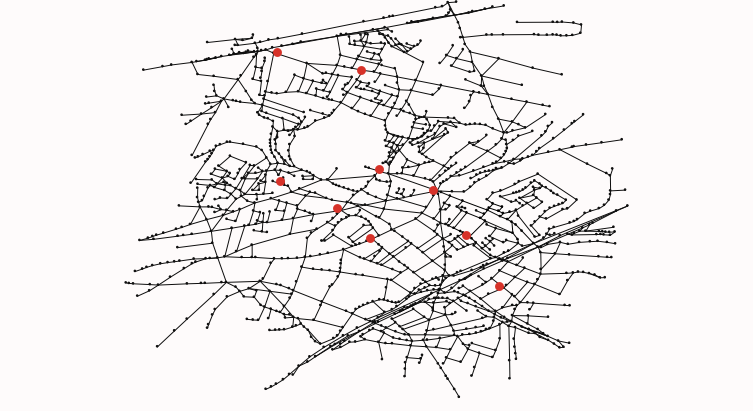
\includegraphics[width=0.45\textwidth]{Figures/PartII/Modeling/NetworkGrowth/tick1}
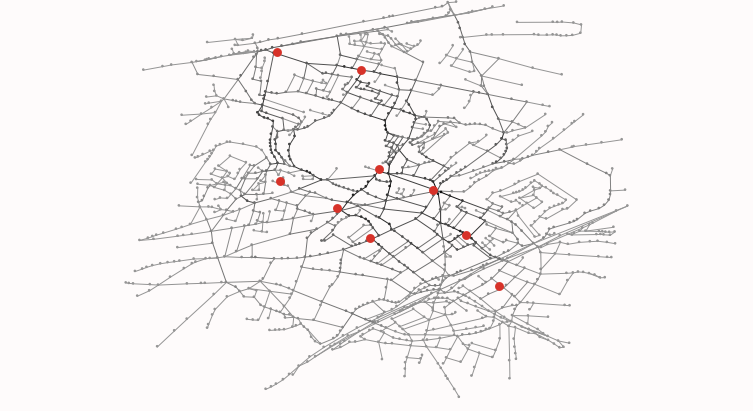
\includegraphics[width=0.45\textwidth]{Figures/PartII/Modeling/NetworkGrowth/tick20}\\
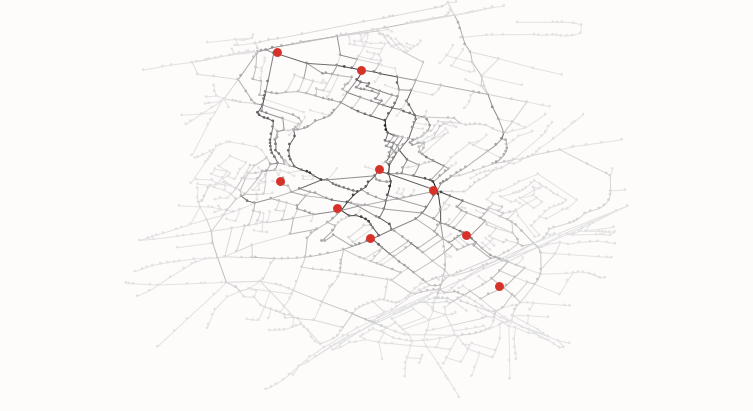
\includegraphics[width=0.45\textwidth]{Figures/PartII/Modeling/NetworkGrowth/tick50}
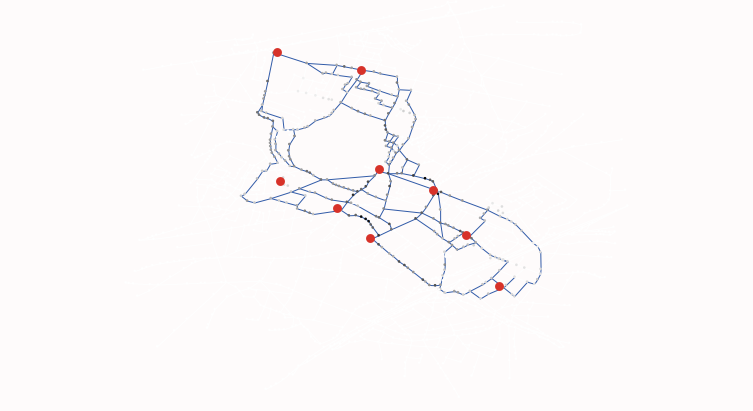
\includegraphics[width=0.45\textwidth]{Figures/PartII/Modeling/NetworkGrowth/reseauFinal}
\caption[Biological Network Growth]{Example of the application of the slime mould network generation model to the computation of an optimal public transportation network design.}
\label{fig:slimemould}
\end{figure}
%%%%%%%%%%%%%%%%%%%%%%%






\subsection{An interdisciplinary approach to network morphogenesis}

An interdisciplinary project that was just launched with a Physicist \noun{Lagesse}, an Architect \noun{Hachi} and a Computer Scientist \noun{Dugue} aims at finding consistent models of urban street network morphogenesis, regarding urban design particularities, geographical rules and complex network indicators feedbacks. Models of network morphogenesis were already discuss here and the aim of this project is to gain insight from the interdisciplinary vision to explore the potentiality of such models. In the frame of our thesis, it is logically situated within the morphogenesis theoretical part and network growth modeling heuristics.












